\begin{minipage}{0.49\linewidth}
    \subsubsection*{Ion-channel-coupled}
        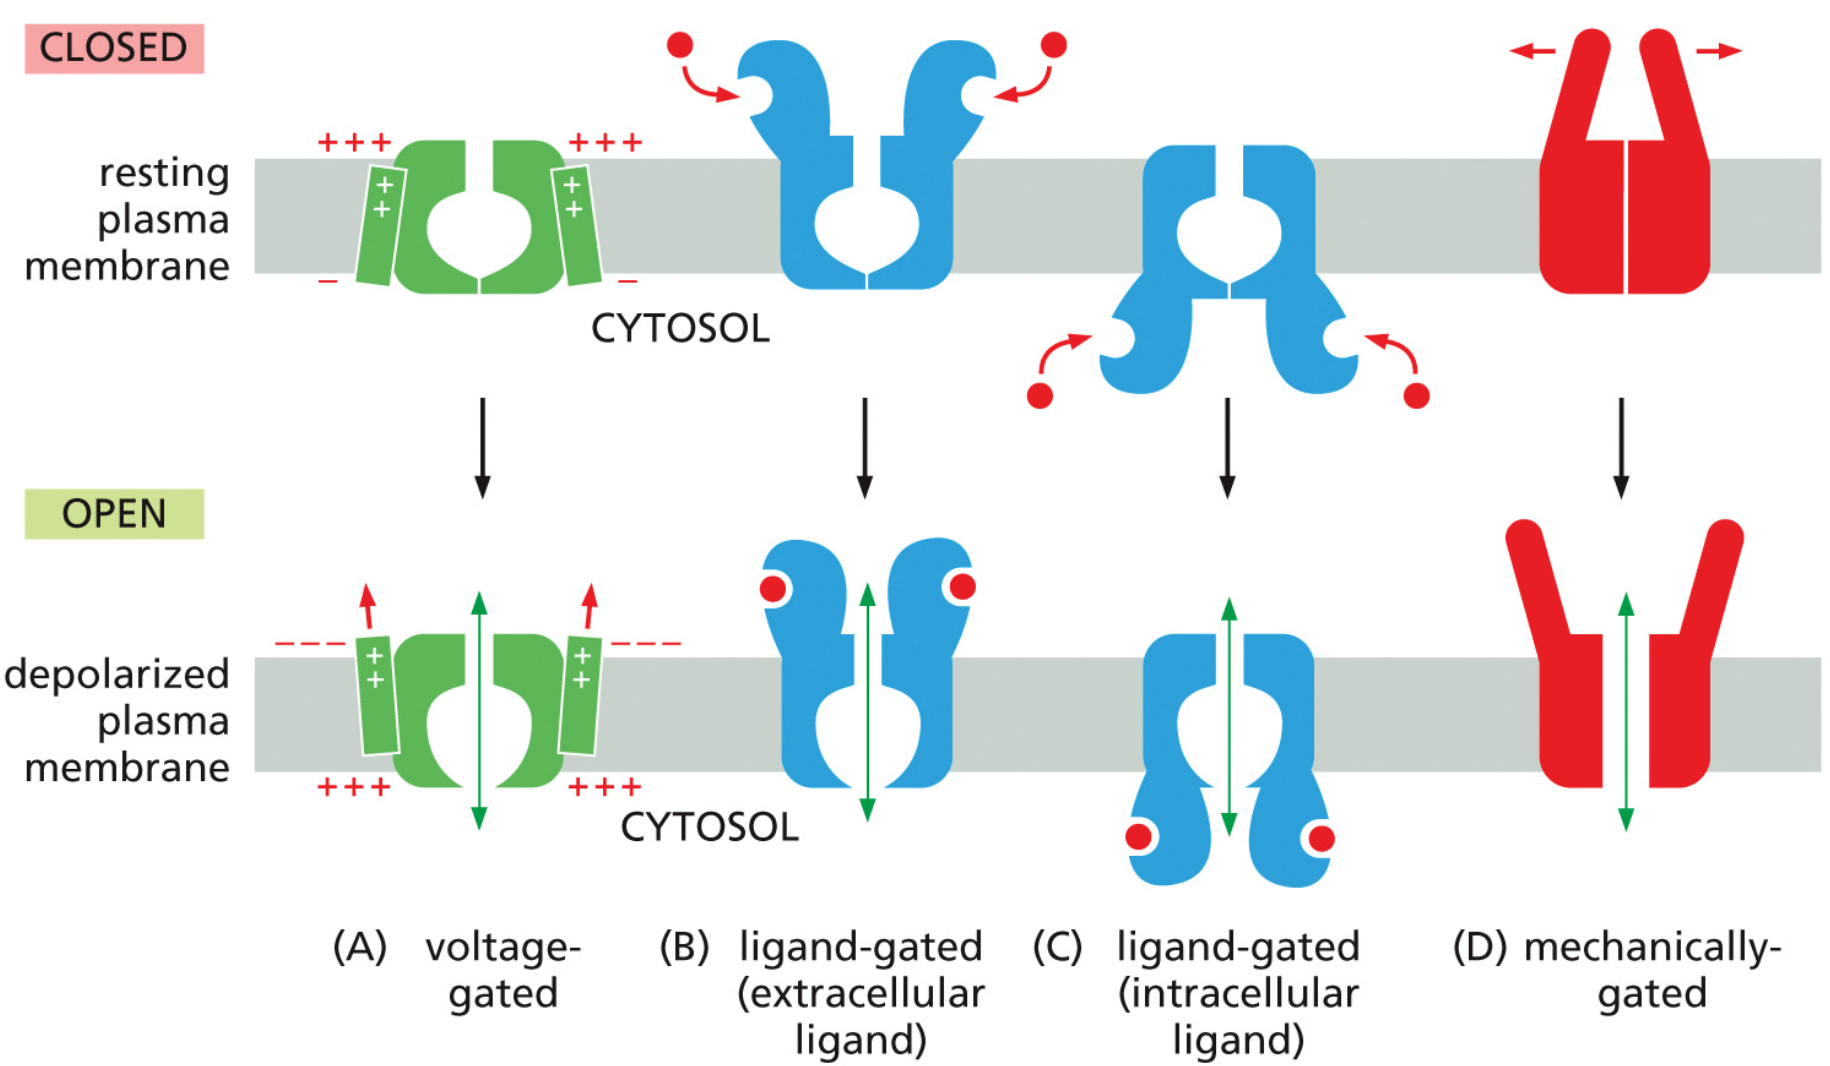
\includegraphics[width=28mm]{src/Images/ion_channel.png}
\end{minipage}
\begin{minipage}{0.49\linewidth}
\subsubsection*{Enzyme-coupled}
    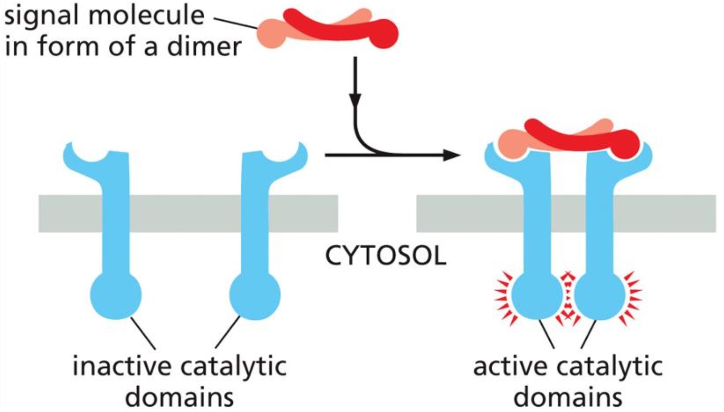
\includegraphics[width=28mm]{src/Images/enzyme_coupled.png}
\end{minipage}

\subsubsection*{G-protein-coupled receptors}
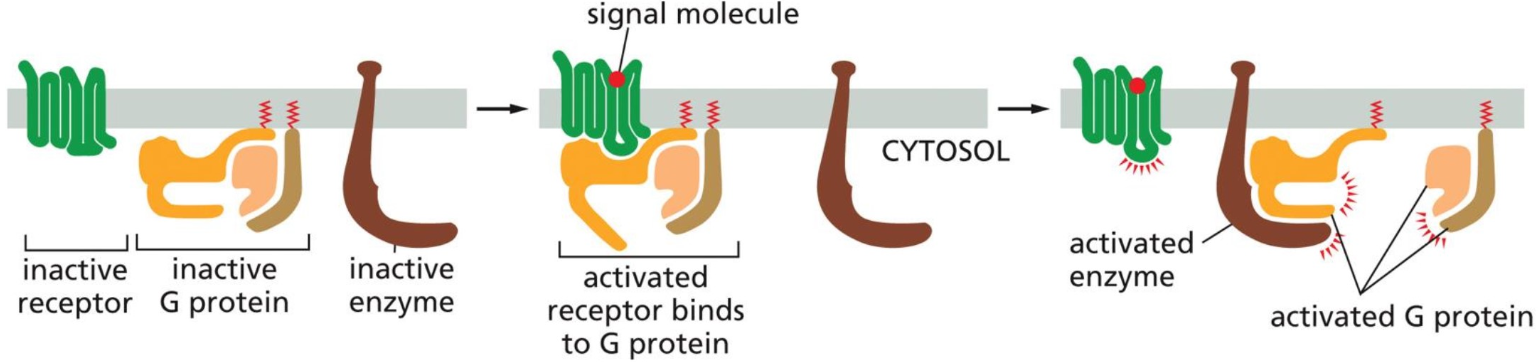
\includegraphics[width=70mm]{src/Images/g_protein.png}

\begin{itemize}
    \item Ligands (ex.: hormones, neurotransmitters) bind to GPCR (G-protein coupled receptor) which changes conformation
    \item Activated receptor causes G-protein to exchange its GDP for GTP gets activated
    \item G-protein modulates the activity of effector molecules generate intracellular second messenger
\end{itemize}

